\documentclass[12pt]{report}

\usepackage{amsmath}
\usepackage{amsfonts}
\usepackage{amssymb}
\usepackage{amsthm}
\usepackage{ulem} % underline
\usepackage{float} % H float specifier
\usepackage{hyperref} % hyperlinks
\usepackage{tabularx} % tabular with column specifier X to break lines
% \usepackage{hyphenat}
\usepackage{bookmark}
\usepackage{systeme} % systems of equation
\usepackage[utf8]{inputenc} % necessary for proper unicode support
\usepackage{parcolumns} % multiple column parallel typesetting
\usepackage[english]{babel} % comment this for Angelsächsisch
\usepackage{graphicx} % including graphics
\usepackage{sourcecodepro} % best font
\usepackage{listings} % source code listings
\usepackage{biblatex} % better citation
% \usepackage[a4paper, top=1cm, left=2cm, right=2cm, includeheadfoot]{geometry} % customize page geometry

% umlauts in lstlistings env
\lstset{
    literate={ö}{{\"o}}1
    {ä}{{\"a}}1
    {ü}{{\"u}}1
    {Ö}{{\"O}}1
    {Ä}{{\"A}}1
    {Ü}{{\"U}}1
}

\lstset{
    basicstyle=\scriptsize\ttfamily,
    breaklines=true
}

\lstset {
    frame=single,
    numbers=left,
    stepnumber=1,
    firstnumber=1,
    numberfirstline=true,
    texcl=false
}

\providecommand{\lxor}{\veebar}
\renewcommand{\proofname}{Beweis.}
\newcommand{\sref}[1]{\textsuperscript{\ref{#1}}}
\newcommand{\F}[1]{\mathbb{F}_2^{#1}}

\addbibresource{refs.bib}

\title{
    \textbf{Efficient Implementation Strategies for Block Ciphers on ARMv8}\\
    {\footnotesize Bachelorarbeit}
}
\author{Bastian Engel}
\date{\today}

\begin{document}

\maketitle

\chapter*{Abstract}

Lorem ipsum dolor \cite{gift:2017} sit amet, consectetur adipisicing elit, sed do eiusmod tempor
incididunt ut labore et dolore magna aliqua. Ut enim ad minim veniam, quis
nostrud exercitation ullamco laboris nisi ut aliquip ex ea commodo consequat.
Duis aute irure dolor in reprehenderit in voluptate velit esse cillum dolore eu
fugiat nulla pariatur. Excepteur sint occaecat cupidatat non proident, sunt in
culpa qui officia deserunt mollit anim id est laborum.

\chapter*{Declaration}

I hereby declare that ...

\tableofcontents

\chapter{Introduction}
\section{Notation}

\section{Block ciphers}

Securing communication channels between different parties has been a long-term
subject of study for cryptographers and engineers which is essential to our
modern world to cope with ever-increasing amounts of devices producing and
sharing data. The main way to facilitate high-throughput, confidential
communications nowadays is through the use of symmetric cryptography in which
two parties share a common secret, called a key, which allows them to encrypt,
share and subsequently decrypt messages to achieve confidentiality against
third parties. Ciphers can be divided into two categories; block ciphers, which
always encrypt fixed-sized messages called blocks, and stream ciphers, which
continuously provide encryption for an arbitrarily long, constant stream of
data.

A block cipher can be defined as a bijection between the input block (the
message) and the output block (the ciphertext). For any block cipher with block
size $n$, we denote the key-dependent encryption and decryption functions as
$E_K,D_K:\F{n}\rightarrow \F{n}$. The simplest way to
characterize this bijection is through a lookup table which yields the highest
possible performance as each block can be encrypted by one simple lookup
depending on the key and the message. This is not practical though due to most
ciphers working with block and key sizes $n,|K|\geq 64$. For a block cipher
with $n=64,|K|=128$, a space of $2^{64}2^{128}64=2^{198}$ is necessary.
Considering modern consumer hard disks being able to store data in the order of
$2^{40}$, it is easy to see that a lookup table is wholly impractical. We
therefore describe block ciphers algorithmically which opens up possibilities
for different tradeoffs and security concerns.


\subsection{GIFT}

\texttt{GIFT}\cite{gift:2017}, first presented in the \textit{CHES 2017}
cryptographic hardware and embedded systems conference, is a lightweight block
cipher based on a previous design called \texttt{PRESENT}, developed in 2007. Its
goal is to offer maximum security while being extremely light on resources.
Modern battery-powered devices like RFID tags or low-latency operations like
on-the-fly disc encryption present strong hardware and power constraints. GIFT
aims to be a simple, low-energy cipher suited for these kinds of applications.

\texttt{GIFT} comes in two variants; \verb|GIFT-64| working with 64-bit blocks
and \texttt{GIFT-128} working with 128-bit blocks. In both cases, the key is 128
bits long. The design is a very simple, round-based substitution-permutation
network (SPN). One round consists in a sequential application of the confusion
layer by means of 4-bit S-boxes and subsequent diffusion through bit
permutation. After the bit permutation, a round key is added to the cipher
state and the single round is complete. \texttt{GIFT-64} uses 28 rounds while
\texttt{GIFT-128} uses 40 rounds.

\begin{figure}[h!]
    \centering
    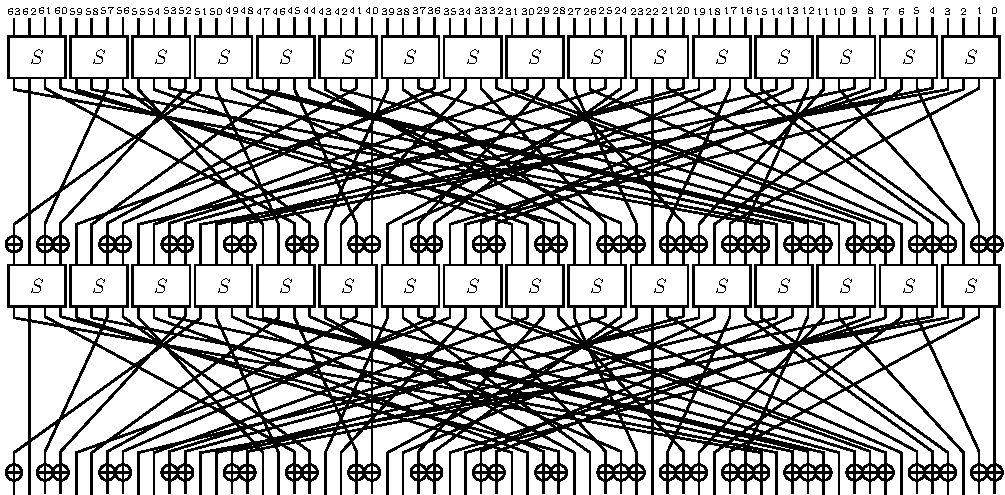
\includegraphics[width=\textwidth]{Figures/GIFT-64.pdf}
    \caption{Two rounds of GIFT-64}
\end{figure}

\subsubsection{Substitution layer}

The input of \texttt{GIFT} is split into 4-bit nibbles which are then fed into
16 S-boxes for \texttt{GIFT-64} and 32 S-boxes for \texttt{GIFT-128}. The S-box
$S:\F{4}\rightarrow \F{4}$ is defined as follows:

\[
    \begin{array}{l|cccccccccccccccc}
        x & 0 & 1 & 2 & 3 & 4 & 5 & 6 & 7 & 8 & 9 & a & b & c & d & e & f \\
        \hline
        S(x) & 1 & a & 4 & c & 6 & f & 3 & 9 & 2 & d & b & 7 & 5 & 0 & 8 & e
    \end{array}
\]

\subsubsection{Permutation layer}

The permutation $P$ works on individual bits and maps bit $b_i$ to $b_{P(i)},
i\in\{0,1,\dots,n-1\}$. The different permutations for \texttt{GIFT-64} and
\texttt{GIFT-128} can be expressed by:

\begin{align*}
    P_{64}(i)&=4\left\lfloor\frac{i}{16}\right\rfloor+16\left(\left(3\left\lfloor\frac{i\bmod 16}{4}\right\rfloor+(i\bmod 4)\right)\bmod 4\right)+(i\bmod 4) \\
    P_{128}(i)&=4\left\lfloor\frac{i}{16}\right\rfloor+32\left(\left(3\left\lfloor\frac{i\bmod 16}{4}\right\rfloor+(i\bmod 4)\right)\bmod 4\right)+(i\bmod 4) \\
\end{align*}

\subsubsection{Round key addition}

The last step of each round consists in XORing a round key $R_i$ to the cipher
state. The new cipher state $s_{i+1}$ after each full round is therefore given
by

\[
    s_{i+1}=P(S(s_i))\oplus R_i
\]

\subsubsection{Round key extraction and key schedule}

Round key extraction differs for \texttt{GIFT-64} and \texttt{GIFT-128}. Let
$K=k7||k6||\dots||k0$ denote the $128$-bit key state.

\paragraph{GIFT-64}. We extract two 16-bit words $U||V=k_1||k_0$ from the key
state. $u_i$ and $v_i$ are XORed to $r_{4i+1}$ and $r_{4i}$ of the round key
$R$ respectively.

\paragraph{GIFT-128}. We extract two 32-bit words $U||V=k_5||k4||k1||k_0$ from
the key state. $u_i$ and $v_i$ are XORed to $r_{4i+2}$ and $b_{4i+1}$ of the
round key $R$ respectively.

In both cases, we additionally XOR a round constant $C=c_5c_4c_3c_2c_1c_0$ to
bit positions $n-1,23,19,15,11,7,3$. The round constants are generated using a
6-bit affine linear-feedback shift register and have the following values:\\

\begin{tabular}{r|l}
    \textbf{Rounds} & \textbf{Constants} \\
    \hline
    \textbf{1 - 16} &  \small\texttt{01,03,07,0F,1F,3E,3D,3B,37,2F,1E,3C,39,33,27,0E} \\
    \textbf{17 - 32} & \small\texttt{1D,3A,35,2B,16,2C,18,30,21,02,05,0B,17,2E,1C,38} \\
    \textbf{33 - 48} & \small\texttt{31,23,06,0D,1B,36,2D,1A,34,29,12,24,08,11,22,04}
\end{tabular}\\

The key state is then updated by setting $k_1\leftarrow k_1\ggg 2$,
$k_0\leftarrow k_0\ggg 12$ and rotating the new state $32$ bits to the right:

\[
    k_7||k_6||\dots||k_1||k_0\leftarrow k_1\ggg 2||k_0\ggg 12||k_7||k_6||\dots||k_3||k_2
\]

\subsection{Camellia}

\section{The ARMv8 platform}

With small devices, embedded processors and ASICs becoming ever more ubiquitous
and essential in areas like medicine or automotive design, the need for ...

\chapter{Implementation strategies}

Due to the structural differences of SPN- and Feistel network-based ciphers, we
shall analyze these two separately.

\section{Strategies for SPN}

Three implementation strategies for substitution-permutation networks are
introduced by \cite{implx86:2014}:

\begin{itemize}
    \item Table-based implementations
    \item \texttt{vperm} implementations
    \item Bitslice implementations
\end{itemize}

\subsection{Table-based}

Table-driven programming is a simple way to increase performance of operations
by tabulating the results, therefore requiring only a single memory access to
acquire the result. This approach is obviously limited to manageable table
sizes, so while tabulating a function like the AES S-box
$S_{AES}:\F{8}\rightarrow \F{8}$ requires only $2^{11}$ space,
tabulating the \texttt{GIFT} permutation layer
$P_{GIFT}:\F{64}\rightarrow \F{64}$ would require
$2^{70}$ space, which is totally unfeasible.

A common approach is to tabulate the output of each S-box, including the
diffusion layer, and then XORing the results together. Let $n$ denote the
internal cipher state size and $s$ the size of a single S-box in bits. For each
S-box $S_i,i\in\{0,\dots,\frac{n}{s}\}$, we can construct a mapping
$T_i:\F{s}\rightarrow \F{n}$ representing substitution with subsequent
permutation of that single S-box. The cipher state before round key addition is
then given by $\bigoplus_{i=0}^{\frac{n}{s}-1}{T_i(m_i)}$ for each $s$-bit
message chunk $m_i$. This approach requires space of
$\frac{n}{s}|\F{s}|n=\frac{n^2 2^s}{s}$ bits, which, for \texttt{GIFT-64},
results in a manageable size of $\frac{64^2 2^4}{4}=2^{14}$ bits which equals
$16$ KiB.

\subsubsection{Constructing the tables}

For \texttt{GIFT-64}, table construction is relatively straightforward and can
be done as follows:

\begin{lstlisting}[caption={Table construction algorithm}, escapechar=|]
    tables <- [][]
    for sbox_index from 0 to 15 do
        for sbox_input from 0 to 15 do|\label{lst:tablesbox}|
            output <- sbox(sbox_input)
            output <- permute(output << (4 * sbox_index))
            tables[sbox_index][sbox_input] <- output
\end{lstlisting}

Implementing this algorithm gives us the following table representing the first
and second S-box.

\[
    \begin{array}{l|l|l|c}
        x & T_0(x) & T_1(x) & \dots \\
        \hline
        0x0 & 0x1               & 0x1000000000000   & \dots \\
        0x1 & 0x8000000020000   & 0x800000002       & \dots \\
        0x2 & 0x400000000       & 0x40000           & \dots \\
        0x3 & 0x8000400000000   & 0x800040000       & \dots \\
        0x4 & 0x400020000       & 0x40002           & \dots \\
        0x5 & 0x8000400020001   & 0x1000800040002   & \dots \\
        0x6 & 0x20001           & 0x1000000000002   & \dots \\
        0x7 & 0x8000000000001   & 0x1000800000000   & \dots \\
        0x8 & 0x20000           & 0x2               & \dots \\
        0x9 & 0x8000400000001   & 0x1000800040000   & \dots \\
        0xa & 0x8000000020001   & 0x1000800000002   & \dots \\
        0xb & 0x400020001       & 0x1000000040002   & \dots \\
        0xc & 0x400000001       & 0x1000000040000   & \dots \\
        0xd & 0x0               & 0x0               & \dots \\
        0xe & 0x8000000000000   & 0x800000000       & \dots \\
        0xf & 0x8000400020000   & 0x800040002       & \dots
    \end{array}
\]

The tables for \texttt{GIFT-128} can be generated in a similar way by looping
through all 32 S-boxes instead of 16 on line \ref{lst:tablesbox}.

\subsection{Using \texttt{vperm}}

Nowadays, most instructions set architectures support single-instruction,
multiple-data processing. The idea of such an SIMD system is to work on
multiple data stored in vectors at once to speed up calculations. For A64, two
types of vector processing are available:

\begin{enumerate}
    \item Advanced SIMD, known as NEON
    \item Scalable Vector Extension (SVE)
\end{enumerate}

We will take a look at NEON as this is the type of vector processing supported
by the Cortex-A73 processor.

\subsubsection{ARM Neon}

The register file of the NEON unit is made up of 32 quad-word (128-bit)
registers \texttt{V[0-31]}, each extending the standard 64-bit floating-point
registers \mbox{\texttt{D[0-31]}}. These registers are divided into equally
sized lanes on which the vector instructions operate. Valid ways to interpret
for example the register \texttt{V0} are:

\begin{figure}[h!]
    \centering
    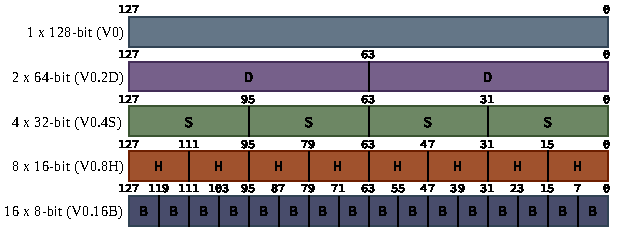
\includegraphics[width=\textwidth]{Figures/V_register.pdf}
    \caption{Divisions of the V0 register}
\end{figure}

NEON instructions interpret their operands' layouts (i.e. lane count and width)
through the use of suffixes such as \texttt{.4S} or \texttt{.8H}. For example,
adding eight 16-bit halfwords from register \texttt{V1} and \texttt{V2}
together and storing the result in \texttt{V0} can be done as follows:

\begin{center}
    \texttt{ADD V0.8H, V1.8H, V2.8H}
\end{center}

\begin{figure}[h!]
    \centering
    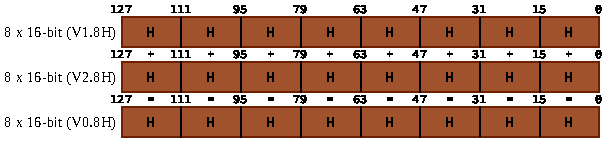
\includegraphics[width=\textwidth]{Figures/vector_add.pdf}
    \caption{Addition of two vector registers}
\end{figure}

The plenitude of different processing instructions allow flexible ways to
further speed up algorithms having reached their optimizational limit on
non-SIMD platforms. \texttt{vperm}, a general term standing for \textit{vector
permute}, is a common instruction on SIMD machines. Called \texttt{TBL} on
NEON, it is used for parallel table lookups and arbitrary permutations. It takes
two inputs to perform a lanewise lookup:

\begin{enumerate}
    \item A register with lookup values
    \item Two or more registers containing data
\end{enumerate}

\subsubsection{S-box lookup}

This instruction can be used to implement S-box lookup of all 16 S-boxes in a
single instruction. We do this by packing our 64-bit cipher state
$s=s_{15}||s_{14}||\dots||s_0$ into a vector register $V_0$. Because we can
only operate on whole bytes, we put each 4-bit S-box into an 8-bit lane which
neatly fits into the 128-bit registers. We then put the S-box itself into
register $V_1$ which will be used as the data register for the table lookup.

The confusion layer can now be performed through one \texttt{TBL} instruction:

\begin{center}
    \texttt{TBL V0.16B, V1.16B, V0.16B}
\end{center}

\begin{figure}[h!]
    \centering
    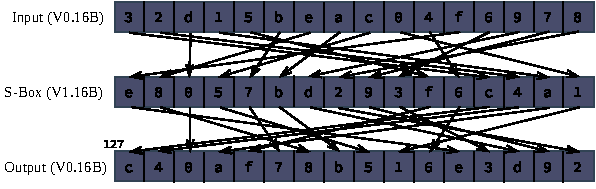
\includegraphics[width=\textwidth]{Figures/tbl_example.pdf}
    \caption{Performing the S-Box lookup in parallel}
\end{figure}

\subsection{Bitslicing}

Bitslicing refers to the technique of splitting up $n$ bits into $m$ slices to
achieve a more efficient representation to operate on. The structure of
\texttt{GIFT} naturally offers possibilities for bitslicing. We split the
cipher state bits $b_{63}b_{62}\dots b_0$ into four slices $S_i,
i\in\{0,1,2,3\}$ such that the $i$-th slice contains all $i$-th bits of the
individual S-boxes. This is equivalent to transposing the bit matrix.

\[
    S=\begin{bmatrix}
        S_0\\
        S_1\\
        S_2\\
        S_3
    \end{bmatrix}
    =\begin{bmatrix}
        b_{60}b_{56}b_{52}\dots b_0\\
        b_{61}b_{57}b_{53}\dots b_1\\
        b_{62}b_{58}b_{54}\dots b_2\\
        b_{63}b_{59}b_{55}\dots b_3
    \end{bmatrix}
\]

\subsubsection{Parallel S-Boxes}

This representation offers multiple advantages. We first note that computation
of the S-box can be executed in parallel, similar to the \texttt{vperm}
technique above. This can be done by finding an algorithmic way to apply the
S-box which has already been proposed by the original \texttt{GIFT} authors:

\begin{align*}
    S_1&\leftarrow S_1\oplus (S_0\land S_2) \\
    t&\leftarrow S_0\oplus (S_1\land S_3) \\
    S_2&\leftarrow S_2\oplus (t\lor S_1) \\
    S_0&\leftarrow S_3\oplus S_2 \\
    S_1&\leftarrow S_1\oplus S_0 \\
    S_0&\leftarrow \lnot S_0 \\
    S_2&\leftarrow S_2\oplus (t\land S_1) \\
    S_3&\leftarrow t
\end{align*}

This is very efficient as it only requires six XOR-, three AND and one OR
operation.

An important property of the permutation is the fact that bits always stay in
their slice. This means we can decompose the permutation $P$ into four
permutations $P_i,i\in\{0,1,2,3\}$ and apply these permutations
separately to each slice. One possible way to implement a permutation $P_i$ in
software is to mask off all bits individually, shift them to their correct
position and OR them together:

\[
    P_i(S_i)=\bigvee_{k=0}^{15}{(S_i\land m_i) \ll s_i}
\]

This approach requires $47$ operations, meaning all four permutations require
over $150$ operations which would present a major bottleneck to the round
function. We can improve on this by working on multiple message blocks at once
and using the aforementioned \texttt{vperm} instruction to implement the bit
shuffling. We then need only four instructions for the complete diffusion
layer.

\subsubsection{Using \texttt{vperm} for slice permutation}

We cannot use the \texttt{TBL} instruction directly as we need to shuffle
individual bits, but the smallest data we can operate on are bytes. We
therefore encrypt $8n$ messages at once which allows us to create bytewise
groupings. These messages are put into $4m$ registers with register $R_{4i}$
containing $S_0$, register $R_{4i+1}$ containing $S_1$ and so forth. With block
size $BS$ and register size $RS$, the following must hold:

\[
    8n\cdot BS=4m\cdot RS
\]

In the case of \texttt{GIFT-64} with $BS=64$ and ARM NEON with $RS=128$, we get

\[
    8n\cdot 64=4m\cdot 128\Leftrightarrow n=m
\]

$n=m=1$ would be a valid choice which yields eight messages divided into four
registers. We choose $n=m=2$ so we can directly utilize the algorithm for bit
packing presented by the original GIFT authors, although it is simple to adapt
this algorithm to only four registers and eight messages by adjusting the
\texttt{SWAPMOVE} shift and mask values.

\subsubsection{Packing the data into bitslice format}

Let $a,b,\dots,p$ be sixteen messages of length $64$ with subscripts denoting
individual bits. We first put these messages into eight SIMD registers
$V_0,V_1,\dots,V_7$:

\begin{alignat*}{3}
    V_0&=b||a\qquad V_4&&=j||&&i \\
    V_1&=d||c\qquad V_5&&=l||&&k \\
    V_2&=f||e\qquad V_6&&=n||&&m \\
    V_3&=h||g\qquad V_7&&=p||&&o
\end{alignat*}

We then use the \texttt{SWAPMOVE} technique to bring the data into bitslice
format. This operation operates on two registers $A,B$ using mask $M$ and shift
value $N$. It swaps bits in $A$ masked by $(M\ll N)$ with bits in $B$ masked by
$M$ in using only three XOR-, one AND- and two shift operations.

\begin{align*}
    &\text{SWAPMOVE}(A,B,M,N): \\
    &\qquad T=((A\gg N)\oplus B)\land M \\
    &\qquad B=B\oplus T \\
    &\qquad A=A\oplus (T\ll N) \\
\end{align*}

One caveat of this approach is the fact that NEON registers cannot be shifted
in their entirety due to the fact bits are not able to cross lanes. This leads
to the problem of being able to shift at most two lanes of 64 bits at once. We
thus need to implement the \texttt{shr(V,n)} and \texttt{shl(V,n)} operations
on our own. This can be done by first extracting the 64-bit lanes $a,b$ out of
$V=b||a$, shifting the lanes individually and finally shifting and ORing the
crossing bits back into the other lane.

\begin{alignat*}{2}
    &\text{shl}(V,n): \\
    &\qquad a,b&&=V[0],V[1] \\
    &\qquad c&&=(a\gg (64-n)) \\
    &\qquad a&&=(a\ll n) \\
    &\qquad b&&=(b\ll n)\lor c \\
    &\qquad V[0],V[1]&&=a,b
\end{alignat*}

The following operations group all $i$th bits of the messages $a,c,\dots,o$
into bytes and puts these into the lower half of the registers $V_{i\bmod 8}$.
The same is done for messages $b,d,\dots,p$, only differing in that the bytes
are put into the upper half of the registers.

\begin{align*}
    &\text{SWAPMOVE}(V_0,V_1,0x5555\dots 55,1) &\text{SWAPMOVE}(V_4,V_5,0x5555\dots 55,1) \\
    &\text{SWAPMOVE}(V_2,V_3,0x5555\dots 55,1) &\text{SWAPMOVE}(V_6,V_7,0x5555\dots 55,1) \\
    &\text{SWAPMOVE}(V_0,V_2,0x3333\dots 33,2) &\text{SWAPMOVE}(V_4,V_6,0x3333\dots 33,2) \\
    &\text{SWAPMOVE}(V_1,V_3,0x3333\dots 33,2) &\text{SWAPMOVE}(V_5,V_7,0x3333\dots 33,2) \\
    &\text{SWAPMOVE}(V_0,V_4,0x0f0f\dots 0f,4) &\text{SWAPMOVE}(V_1,V_5,0x0f0f\dots 0f,4) \\
    &\text{SWAPMOVE}(V_2,V_6,0x0f0f\dots 0f,4) &\text{SWAPMOVE}(V_3,V_7,0x0f0f\dots 0f,4) \\
\end{align*}

With $Ax=o_xm_xk_xj_xg_xe_xc_xa_x$ and $Bx=p_xn_xl_xi_xh_xf_xd_xb_x$ denoting
byte groups, our data now has the following permutation-friendly format:

\[
    \scriptsize
    \begin{array}{c|llllllll|llllllll}
        n & 15 & 14 & 13 & 12 & 11 & 10 & 9 & 8 & 7 & 6 & 5 & 4 & 3 & 2 & 1 & 0 \\
        \hline
        V_0 & B56 & B48 & B40 & B32 & B24 & B16 & B8 & B0 & A56 & A48 & A40 & A32 & A24 & A16 & A8 & A0 \\
        V_1 & B57 & B49 & B41 & B33 & B25 & B17 & B9 & B1 & A57 & A49 & A41 & A33 & A25 & A17 & A9 & A1 \\
        V_2 & B58 & B50 & B42 & B34 & B26 & B18 & B10 & B2 & A58 & A50 & A42 & A34 & A26 & A18 & A10 & A2 \\
        V_3 & B59 & B51 & B43 & B35 & B27 & B19 & B11 & B3 & A59 & A51 & A43 & A35 & A27 & A19 & A11 & A3 \\
        V_4 & B60 & B52 & B44 & B36 & B28 & B20 & B12 & B4 & A60 & A52 & A44 & A36 & A28 & A20 & A12 & A4 \\
        V_5 & B61 & B53 & B45 & B37 & B29 & B21 & B13 & B5 & A61 & A53 & A45 & A37 & A29 & A21 & A13 & A5 \\
        V_6 & B62 & B54 & B46 & B38 & B30 & B22 & B14 & B6 & A62 & A54 & A46 & A38 & A30 & A22 & A14 & A6 \\
        V_7 & B63 & B55 & B47 & B39 & B31 & B23 & B15 & B7  & A63 & A55 & A47 & A39 & A31 & A23 & A15 & A7
    \end{array}
\]

Although this would already work, we prefer to have only bits of the same
messages in each register - otherwise the permutation would need to operate on
two source registers with the added requirement of storing the pre-permutation
values for the first four registers, slowing down the round function through
superfluous load/stores. This transformation is trivial by use of
\texttt{TBL} with two data source operands.

We can now create permutation tables using the specification of the individual
slice permutations $P_i$:

\[
    \begin{array}{c|llllllllllllllll}
        j & 0 & 1 & 2 & 3 & 4 & 5 & 6 & 7 & 8 & 9 & 10 & 11 & 12 & 13 & 14 & 15 \\
        \hline
        P_0(j) & 0 & 12 & 8 & 4 & 1 & 13 & 9 & 5 & 2 & 14 & 10 & 6 & 3 & 15 & 11 & 7 \\
        P_1(j) & 4 & 0 & 12 & 8 & 5 & 1 & 13 & 9 & 6 & 2 & 14 & 10 & 7 & 3 & 15 & 11 \\
        P_2(j) & 8 & 4 & 0 & 12 & 9 & 5 & 1 & 13 & 10 & 6 & 2 & 14 & 11 & 7 & 3 & 15 \\
        P_3(j) & 12 & 8 & 4 & 0 & 13 & 9 & 5 & 1 & 14 & 10 & 6 & 2 & 15 & 11 & 7 & 3
    \end{array}
\]

Another thing to take note of is the original permutation values only showing
where a given byte should land, not which byte belongs to a certain position -
i.e. for $P_0$, byte 1 should land in position 12, but the byte belonging to
position 1 is byte 4. Because \texttt{TBL} works in the latter way, we have
to do some trivial rearrangements.

Assuming the correct permutation values are put into registers
$V_8,V_{10},\dots,V_{15}$, this now allows us to compute the permutation layer
for all 16 blocks in only eight permutation instructions.

\begin{alignat*}{2}
    &\texttt{TBL V0, V0, V8}\qquad &&\texttt{TBL V1, V1, V9} \\
    &\texttt{TBL V2, V2, V10}\qquad &&\texttt{TBL V3, V3, V11} \\
    &\texttt{TBL V4, V4, V12}\qquad &&\texttt{TBL V5, V5, V13} \\
    &\texttt{TBL V6, V6, V14}\qquad &&\texttt{TBL V7, V7, V15}
\end{alignat*}

\subsubsection{Round key function}

In contrast to packing and unpacking of data which is only done once in the
beginning and end, a round key is derived for every round, so the round key
derivation function needs to be as fast as possible. A simple but naive
approach for one round would be to generate a single round key, copy it 15
times and pack the resulting registers similar to how we proceed with the
messages. Due to the cost of packing the messages, this is prohibitivly
expensive. Because we know where each byte group ends up after packing, we can
directly set the round key bits at the correct position. Extending these bits
to bytes can then be done simply by repeatedly shifting and ORing the registers
together.

\subsection{Strategies for Camellia}

\chapter{Implementation}

We will provide and discuss implementations for the presented strategies in the
C programming language. Although directly writing Assembler code could result
in a small performance benefit, this generally increases the work necessary by
an order of magnitude for only limited results. This is why we use NEON
intrinsics.

\subsection{NEON intrinsics}

The header file \texttt{<arm\_neon.h>} provides ARM-specific data and function
definitions including vector data types and C functions for working with these
vectors. These functions are known as NEON intrinsics and give the programmer a
high-level interface to most NEON instructions. Major advantages of this
approach include the ease of development as the compiler takes over register
allocation and load/store operations as well as performance benefits through
compiler optimizations.

Standard vector data types have the format \texttt{uintnxm\_t} with lane width
$n$ in bits and and lane count $m$. Array types of the format
\texttt{uintnxmxc\_t}, $c\in\{2,3,4\}$ are also defined which are used in
operations requiring multiple parameters like \texttt{TBL} or pairwise
load/stores. Intrinsics start with \texttt{v}, optionally contain a \texttt{q}
after the operation name to indicate operation on a 128-bit register, and end
with the lane data format. Multiplying eight pairs of 16-bit numbers
\texttt{a,b} for example can be done via the following:

\begin{center}
    \texttt{uint16x8\_t result = vmulq\_u16(a, b);}
\end{center}

In this case, the compiler allocates vector registers for \texttt{a},
\texttt{b} and \texttt{result} and assembles the intrinsic to \texttt{MUL
Vr.8H, Va.8H, Vb.8H}. Necessary load and stores for the result and parameters
are also handled automatically. Of special interest to us are the following
intrinsics, each existing in different variants with different lane widths and
also array types: \\

\begin{table}[h!]
    \centering
    \footnotesize
    \begin{tabularx}{\textwidth}{ll|X}
        Intrinsic && Description \\
        \hline
        \texttt{uint8x16\_t} & \texttt{vreinterpretq\_u8\_u64(uint64x2\_t)} & Explicit casting \\
        \hline
        \texttt{uint64\_t} & \texttt{vgetq\_lane\_u64(void)} & Extract a single lane \\
        \hline
        \texttt{void} & \texttt{vsetq\_lane\_u64(uint64\_t)} & Insert a single lane \\
        \hline
        \texttt{uint64x2\_t} & \texttt{vdupq\_n\_u64(uint64\_t)} & Initialize all lanes to same value \\
        \hline
        \texttt{void} & \texttt{vst1q\_u64(uint64\_t*, uint64x2\_t)} & Store from register to memory \\
        \hline
        \texttt{uint64x2\_t} & \texttt{vld1q\_u64(uint64\_t*, uint64x2\_t)} & Load from memory to register \\
        \hline
        \texttt{uint8x16\_t} & \texttt{veorq\_u8(uint8x16\_t, uint8x16\_t)} & bitwise XOR \\
        \hline
        \texttt{uint8x16\_t} & \texttt{vandq\_u8(uint8x16\_t, uint8x16\_t)} & bitwise AND \\
        \hline
        \texttt{uint8x16\_t} & \texttt{vorrq\_u8(uint8x16\_t, uint8x16\_t)} & bitwise OR \\
        \hline
        \texttt{uint8x16\_t} & \texttt{vmvnq\_u8(uint8x16\_t)} & bitwise NOT \\
        \hline
        \texttt{uint8x16\_t} & \texttt{vqtbl2q\_u8(uint8x16\_t, uint8x16\_t)} & permutation (\texttt{TBL}) \\
    \end{tabularx}
\end{table}

The implementations closely follow the aforementioned strategies;
instruction-level optimization is left to the compiler.

\chapter{Evaluation}

\chapter{Appendix}

\begin{lstlisting}[language=c, caption={gift\_vec\_sliced.h}]
#ifndef GIFT_VEC_SLICED_H
#define GIFT_VEC_SLICED_H

#include <stdint.h>
#include <arm_neon.h>

#define ROUNDS_GIFT_64 28

// expose for benchmarking
uint8x16_t shl(uint8x16_t v, int n);
uint8x16_t shr(uint8x16_t v, int n);
void gift_64_vec_sliced_swapmove(uint8x16_t *restrict a, uint8x16_t *restrict b,
                                 uint8x16_t m, int n);
void gift_64_vec_sliced_bits_pack(uint8x16x4_t m[restrict 2]);

void gift_64_vec_sliced_subcells(uint8x16x4_t cipher_state[restrict 2]);
void gift_64_vec_sliced_subcells_inv(uint8x16x4_t cipher_state[restrict 2]);
void gift_64_vec_sliced_permute(uint8x16x4_t cipher_state[restrict 2]);
void gift_64_vec_sliced_permute_inv(uint8x16x4_t cipher_state[2]);
void gift_64_vec_sliced_generate_round_keys(uint8x16x4_t round_keys[restrict ROUNDS_GIFT_64][2],
                                            const uint64_t key[restrict 2]);

void gift_64_vec_sliced_init(void);

void gift_64_vec_sliced_encrypt(uint64_t c[restrict 16],
                                const uint64_t m[restrict 16],
                                const uint64_t key[restrict 2]);
void gift_64_vec_sliced_decrypt(uint64_t m[restrict 16],
                                const uint64_t c[restrict 16],
                                const uint64_t key[restrict 2]);

#endif
\end{lstlisting}

\begin{lstlisting}[language=c, caption={gift\_vec\_sliced.c}]
#include "gift_vec_sliced.h"

#include <stddef.h>
#include <stdio.h>
#include <string.h>

static uint64_t perm_u64[16] = {
        0x1410050115110400UL, 0x1410050115110400UL,
        0x0501151104001410UL, 0x0501151104001410UL,
        0x1511040014100501UL, 0x1511040014100501UL,
        0x0400141005011511UL, 0x0400141005011511UL,
        0x1612070317130602UL, 0x1612070317130602UL,
        0x0703171306021612UL, 0x0703171306021612UL,
        0x1713060216120703UL, 0x1713060216120703UL,
        0x0602161207031713UL, 0x0602161207031713UL
};

static uint64_t perm_inv_u64[16] = {
        0x1511050114100400UL, 0x1511050114100400UL,
        0x1713070316120602UL, 0x1713070316120602UL,
        0x1115010510140004UL, 0x1115010510140004UL,
        0x1317030712160206UL, 0x1317030712160206UL,
        0x1317030712160206UL, 0x1317030712160206UL,
        0x1511050114100400UL, 0x1511050114100400UL,
        0x1713070316120602UL, 0x1713070316120602UL,
        0x1115010510140004UL, 0x1115010510140004UL
};

static uint8x16x4_t perm[2];
static uint8x16x4_t perm_inv[2];

static uint8x16_t pack_mask_0;
static uint8x16_t pack_mask_1;
static uint8x16_t pack_mask_2;

static const int round_constant[] = {
        // rounds 0-15
        0x01, 0x03, 0x07, 0x0F, 0x1F, 0x3E, 0x3D, 0x3B,
        0x37, 0x2F, 0x1E, 0x3C, 0x39, 0x33, 0x27, 0x0E,
        // rounds 16-31
        0x1D, 0x3A, 0x35, 0x2B, 0x16, 0x2C, 0x18, 0x30,
        0x21, 0x02, 0x05, 0x0B, 0x17, 0x2E, 0x1C, 0x38,
        // rounds 32-47
        0x31, 0x23, 0x06, 0x0D, 0x1B, 0x36, 0x2D, 0x1A,
        0x34, 0x29, 0x12, 0x24, 0x08, 0x11, 0x22, 0x04
};

uint8x16_t shl(uint8x16_t v, int n)
{
        uint64_t l[2];
        vst1q_u64(l, v);
        l[1] = l[1] << n | (l[0] >> (64 - n));
        l[1] <<= n;
        return vreinterpretq_u8_u64(vld1q_u64(l));
}

uint8x16_t shr(uint8x16_t v, int n)
{
        uint64_t l[2];
        vst1q_u64(l, v);
        l[0] = l[0] >> n | (((l[1] << (64 - n)) >> (64 - n)) << (64 - n));
        l[1] >>= n;
        return vreinterpretq_u8_u64(vld1q_u64(l));
}

void gift_64_vec_sliced_swapmove(uint8x16_t *restrict a, uint8x16_t *restrict b, uint8x16_t m, int n)
{

        uint8x16_t t = vandq_u8(veorq_u8(shr(*a, n), *b), m);
        *b = veorq_u8(*b, t);
        *a = veorq_u8(*a, shl(t, n));
}

void gift_64_vec_sliced_bits_pack(uint8x16x4_t m[restrict 2])
{
        // take care not to shift mask bits out of the register
        gift_64_vec_sliced_swapmove(&m[0].val[0], &m[0].val[1], pack_mask_0, 1);
        gift_64_vec_sliced_swapmove(&m[0].val[2], &m[0].val[3], pack_mask_0, 1);
        gift_64_vec_sliced_swapmove(&m[1].val[0], &m[1].val[1], pack_mask_0, 1);
        gift_64_vec_sliced_swapmove(&m[1].val[2], &m[1].val[3], pack_mask_0, 1);

        gift_64_vec_sliced_swapmove(&m[0].val[0], &m[0].val[2], pack_mask_1, 2);
        gift_64_vec_sliced_swapmove(&m[0].val[1], &m[0].val[3], pack_mask_1, 2);
        gift_64_vec_sliced_swapmove(&m[1].val[0], &m[1].val[2], pack_mask_1, 2);
        gift_64_vec_sliced_swapmove(&m[1].val[1], &m[1].val[3], pack_mask_1, 2);

        // make bytes (a0 b0 c0 d0 a4 b4 c4 d4 -> a0 b0 c0 d0 e0 f0 g0 h0)
        gift_64_vec_sliced_swapmove(&m[0].val[0], &m[1].val[0], pack_mask_2, 4);
        gift_64_vec_sliced_swapmove(&m[0].val[2], &m[1].val[2], pack_mask_2, 4);
        gift_64_vec_sliced_swapmove(&m[0].val[1], &m[1].val[1], pack_mask_2, 4);
        gift_64_vec_sliced_swapmove(&m[0].val[3], &m[1].val[3], pack_mask_2, 4);
}

void gift_64_vec_sliced_subcells(uint8x16x4_t cs[restrict 2])
{
        cs[0].val[1] = veorq_u8(cs[0].val[1], vandq_u8(cs[0].val[0], cs[0].val[2]));
        uint8x16_t t = veorq_u8(cs[0].val[0], vandq_u8(cs[0].val[1], cs[0].val[3]));
        cs[0].val[2] = veorq_u8(cs[0].val[2], vorrq_u8(t, cs[0].val[1]));
        cs[0].val[0] = veorq_u8(cs[0].val[3], cs[0].val[2]);
        cs[0].val[1] = veorq_u8(cs[0].val[1], cs[0].val[0]);
        cs[0].val[0] = vmvnq_u8(cs[0].val[0]);
        cs[0].val[2] = veorq_u8(cs[0].val[2], vandq_u8(t, cs[0].val[1]));
        cs[0].val[3] = t;

        cs[1].val[1] = veorq_u8(cs[1].val[1], vandq_u8(cs[1].val[0], cs[1].val[2]));
        t            = veorq_u8(cs[1].val[0], vandq_u8(cs[1].val[1], cs[1].val[3]));
        cs[1].val[2] = veorq_u8(cs[1].val[2], vorrq_u8(t, cs[1].val[1]));
        cs[1].val[0] = veorq_u8(cs[1].val[3], cs[1].val[2]);
        cs[1].val[1] = veorq_u8(cs[1].val[1], cs[1].val[0]);
        cs[1].val[0] = vmvnq_u8(cs[1].val[0]);
        cs[1].val[2] = veorq_u8(cs[1].val[2], vandq_u8(t, cs[1].val[1]));
        cs[1].val[3] = t;
}

void gift_64_vec_sliced_subcells_inv(uint8x16x4_t cs[restrict 2])
{
        uint8x16_t t = cs[0].val[3];
        cs[0].val[2] = veorq_u8(cs[0].val[2], vandq_u8(t, cs[0].val[1]));
        cs[0].val[0] = vmvnq_u8(cs[0].val[0]);
        cs[0].val[1] = veorq_u8(cs[0].val[1], cs[0].val[0]);
        cs[0].val[3] = veorq_u8(cs[0].val[0], cs[0].val[2]);
        cs[0].val[2] = veorq_u8(cs[0].val[2], vorrq_u8(t, cs[0].val[1]));
        cs[0].val[0] = veorq_u8(t, vandq_u8(cs[0].val[1], cs[0].val[3]));
        cs[0].val[1] = veorq_u8(cs[0].val[1], vandq_u8(cs[0].val[0], cs[0].val[2]));

        t            = cs[1].val[3];
        cs[1].val[2] = veorq_u8(cs[1].val[2], vandq_u8(t, cs[1].val[1]));
        cs[1].val[0] = vmvnq_u8(cs[1].val[0]);
        cs[1].val[1] = veorq_u8(cs[1].val[1], cs[1].val[0]);
        cs[1].val[3] = veorq_u8(cs[1].val[0], cs[1].val[2]);
        cs[1].val[2] = veorq_u8(cs[1].val[2], vorrq_u8(t, cs[1].val[1]));
        cs[1].val[0] = veorq_u8(t, vandq_u8(cs[1].val[1], cs[1].val[3]));
        cs[1].val[1] = veorq_u8(cs[1].val[1], vandq_u8(cs[1].val[0], cs[1].val[2]));
}

void gift_64_vec_sliced_permute(uint8x16x4_t cs[restrict 2])
{
        uint8x16x2_t pairs[4] = {
                { .val = { cs[0].val[0], cs[1].val[0] }},
                { .val = { cs[0].val[1], cs[1].val[1] }},
                { .val = { cs[0].val[2], cs[1].val[2] }},
                { .val = { cs[0].val[3], cs[1].val[3] }},
        };

        cs[0].val[0] = vqtbl2q_u8(pairs[0], perm[0].val[0]);
        cs[0].val[1] = vqtbl2q_u8(pairs[1], perm[0].val[1]);
        cs[0].val[2] = vqtbl2q_u8(pairs[2], perm[0].val[2]);
        cs[0].val[3] = vqtbl2q_u8(pairs[3], perm[0].val[3]);

        cs[1].val[0] = vqtbl2q_u8(pairs[0], perm[1].val[0]);
        cs[1].val[1] = vqtbl2q_u8(pairs[1], perm[1].val[1]);
        cs[1].val[2] = vqtbl2q_u8(pairs[2], perm[1].val[2]);
        cs[1].val[3] = vqtbl2q_u8(pairs[3], perm[1].val[3]);
}

void gift_64_vec_sliced_permute_inv(uint8x16x4_t cs[restrict 2])
{
        uint8x16x2_t pairs[4] = {
                { .val = { cs[0].val[0], cs[1].val[0] }},
                { .val = { cs[0].val[1], cs[1].val[1] }},
                { .val = { cs[0].val[2], cs[1].val[2] }},
                { .val = { cs[0].val[3], cs[1].val[3] }},
        };

        cs[0].val[0] = vqtbl2q_u8(pairs[0], perm_inv[0].val[0]);
        cs[0].val[1] = vqtbl2q_u8(pairs[1], perm_inv[0].val[1]);
        cs[0].val[2] = vqtbl2q_u8(pairs[2], perm_inv[0].val[2]);
        cs[0].val[3] = vqtbl2q_u8(pairs[3], perm_inv[0].val[3]);

        cs[1].val[0] = vqtbl2q_u8(pairs[0], perm_inv[1].val[0]);
        cs[1].val[1] = vqtbl2q_u8(pairs[1], perm_inv[1].val[1]);
        cs[1].val[2] = vqtbl2q_u8(pairs[2], perm_inv[1].val[2]);
        cs[1].val[3] = vqtbl2q_u8(pairs[3], perm_inv[1].val[3]);
}

void gift_64_vec_sliced_generate_round_keys(uint8x16x4_t round_keys[restrict ROUNDS_GIFT_64][2],
                                            const uint64_t key[restrict 2])
{
        // TODO shift-and-or

        uint64_t key_state[] = {key[0], key[1]};
        for (int round = 0; round < ROUNDS_GIFT_64; round++) {
                int v = (key_state[0] >> 0 ) & 0xffff;
                int u = (key_state[0] >> 16) & 0xffff;

                // add round key (RK=U||V)
                uint64_t round_key[8] = { 0x0UL };
                for (size_t i = 0; i < 8; i++) {
                        int key_bit_v   = (v >> (2 * i + 0)) & 0x1;
                        int key_bit_u   = (u >> (2 * i + 0)) & 0x1;
                        round_key[0] ^= (uint64_t)key_bit_v << (i * 8);
                        round_key[1] ^= (uint64_t)key_bit_u << (i * 8);

                        key_bit_v   = (v >> (2 * i + 1)) & 0x1;
                        key_bit_u   = (u >> (2 * i + 1)) & 0x1;
                        round_key[4] ^= (uint64_t)key_bit_v << (i * 8);
                        round_key[5] ^= (uint64_t)key_bit_u << (i * 8);
                }

                // add single bit
                round_key[7] ^= 1UL << (7 * 8);

                // add round constants
                round_key[3] ^= ((round_constant[round] >> 0) & 0x1) << (0 * 8);
                round_key[7] ^= ((round_constant[round] >> 1) & 0x1) << (0 * 8);
                round_key[3] ^= ((round_constant[round] >> 2) & 0x1) << (1 * 8);
                round_key[7] ^= ((round_constant[round] >> 3) & 0x1) << (1 * 8);
                round_key[3] ^= ((round_constant[round] >> 4) & 0x1) << (2 * 8);
                round_key[7] ^= ((round_constant[round] >> 5) & 0x1) << (2 * 8);

                // extend bits to bytes
                for (size_t i = 0; i < 8; i++) {
                        round_key[i] |= round_key[i] << 1;
                        round_key[i] |= round_key[i] << 2;
                        round_key[i] |= round_key[i] << 4;
                }

                // load into vector registers (upper and lower part are same)
                round_keys[round][0].val[0] = vdupq_n_u64(round_key[0]);
                round_keys[round][0].val[1] = vdupq_n_u64(round_key[1]);
                round_keys[round][0].val[2] = vdupq_n_u64(round_key[2]);
                round_keys[round][0].val[3] = vdupq_n_u64(round_key[3]);
                round_keys[round][1].val[0] = vdupq_n_u64(round_key[4]);
                round_keys[round][1].val[1] = vdupq_n_u64(round_key[5]);
                round_keys[round][1].val[2] = vdupq_n_u64(round_key[6]);
                round_keys[round][1].val[3] = vdupq_n_u64(round_key[7]);

                // update key state
                int k0 = (key_state[0] >> 0 ) & 0xffffUL;
                int k1 = (key_state[0] >> 16) & 0xffffUL;
                k0 = (k0 >> 12) | ((k0 & 0xfff) << 4);
                k1 = (k1 >> 2 ) | ((k1 & 0x3  ) << 14);
                key_state[0] >>= 32;
                key_state[0] |= (key_state[1] & 0xffffffffUL) << 32;
                key_state[1] >>= 32;
                key_state[1] |= ((uint64_t)k0 << 32) | ((uint64_t)k1 << 48);
        }
}

void gift_64_vec_sliced_init(void)
{
        // permutations
        perm[0] = vld1q_u8_x4((uint8_t*)&perm_u64[0]);
        perm[1] = vld1q_u8_x4((uint8_t*)&perm_u64[8]);

        // inverse permutations
        perm_inv[0] = vld1q_u8_x4((uint8_t*)&perm_inv_u64[0]);
        perm_inv[1] = vld1q_u8_x4((uint8_t*)&perm_inv_u64[8]);

        // packing masks
        pack_mask_0 = vdupq_n_u8(0x55);
        pack_mask_1 = vdupq_n_u8(0x33);
        pack_mask_2 = vdupq_n_u8(0x0f);
}

void gift_64_vec_sliced_encrypt(uint64_t c[restrict 16],
                                const uint64_t m[restrict 16],
                                const uint64_t key[restrict 2])
{
        uint8x16x4_t s[2];
        s[0] = vld1q_u8_x4((uint8_t*)&m[0]);
        s[1] = vld1q_u8_x4((uint8_t*)&m[8]);
        gift_64_vec_sliced_bits_pack(s);

        uint8x16x4_t round_keys[ROUNDS_GIFT_64][2];
        gift_64_vec_sliced_generate_round_keys(round_keys, key);

        for (int round = 0; round < ROUNDS_GIFT_64; round++) {
                gift_64_vec_sliced_subcells(s);
                gift_64_vec_sliced_permute(s);

                s[0].val[0] = veorq_u8(s[0].val[0], round_keys[round][0].val[0]);
                s[0].val[1] = veorq_u8(s[0].val[1], round_keys[round][0].val[1]);
                s[0].val[2] = veorq_u8(s[0].val[2], round_keys[round][0].val[2]);
                s[0].val[3] = veorq_u8(s[0].val[3], round_keys[round][0].val[3]);
                s[1].val[0] = veorq_u8(s[1].val[0], round_keys[round][1].val[0]);
                s[1].val[1] = veorq_u8(s[1].val[1], round_keys[round][1].val[1]);
                s[1].val[2] = veorq_u8(s[1].val[2], round_keys[round][1].val[2]);
                s[1].val[3] = veorq_u8(s[1].val[3], round_keys[round][1].val[3]);
        }

        gift_64_vec_sliced_bits_pack(s);
        vst1q_u8_x4((uint8_t*)&c[0], s[0]);
        vst1q_u8_x4((uint8_t*)&c[8], s[1]);
}

void gift_64_vec_sliced_decrypt(uint64_t m[restrict 16],
                                const uint64_t c[restrict 16],
                                const uint64_t key[restrict 2])
{
        uint8x16x4_t s[2];
        s[0] = vld1q_u8_x4((uint8_t*)&c[0]);
        s[1] = vld1q_u8_x4((uint8_t*)&c[8]);
        gift_64_vec_sliced_bits_pack(s);

        uint8x16x4_t round_keys[ROUNDS_GIFT_64][2];
        gift_64_vec_sliced_generate_round_keys(round_keys, key);

        for (int round = ROUNDS_GIFT_64 - 1; round >= 0; round--) {
                s[0].val[0] = veorq_u8(s[0].val[0], round_keys[round][0].val[0]);
                s[0].val[1] = veorq_u8(s[0].val[1], round_keys[round][0].val[1]);
                s[0].val[2] = veorq_u8(s[0].val[2], round_keys[round][0].val[2]);
                s[0].val[3] = veorq_u8(s[0].val[3], round_keys[round][0].val[3]);
                s[1].val[0] = veorq_u8(s[1].val[0], round_keys[round][1].val[0]);
                s[1].val[1] = veorq_u8(s[1].val[1], round_keys[round][1].val[1]);
                s[1].val[2] = veorq_u8(s[1].val[2], round_keys[round][1].val[2]);
                s[1].val[3] = veorq_u8(s[1].val[3], round_keys[round][1].val[3]);

                gift_64_vec_sliced_permute_inv(s);
                gift_64_vec_sliced_subcells_inv(s);
        }

        gift_64_vec_sliced_bits_pack(s);
        vst1q_u8_x4((uint8_t*)&m[0], s[0]);
        vst1q_u8_x4((uint8_t*)&m[8], s[1]);
}
\end{lstlisting}

\chapter*{Acknowledgements}

I want to thank ...

\printbibliography

\end{document}
